\documentclass[12pt]{article}

\usepackage[a4paper,left=25mm,right=25mm,top=35mm,bottom=25mm]{geometry}
\usepackage{ngerman}
\usepackage{parskip}
\usepackage{times}
\usepackage{graphicx}
\usepackage{listings}
\usepackage{fancyhdr}
\usepackage{float}
\usepackage{amsmath}

\setlength{\headheight}{15.2pt}
\pagestyle{fancy}

\lhead{Bildverarbeitung und Mustererkennung\\Praktikum Blatt 5}
\rhead{Patrick Hüntelmann\\20.05.2022}

\lstset{
  basicstyle=\ttfamily,
  breakatwhitespace=false,         % sets if automatic breaks should only happen at whitespace
  breaklines=true,                 % sets automatic line breaking
  captionpos=b,                    % sets the caption-position to bottom
  deletekeywords={...},            % if you want to delete keywords from the given language
  escapeinside={\%*}{*)},          % if you want to add LaTeX within your code
  extendedchars=true,              % lets you use non-ASCII characters; for 8-bits encodings only, does not work with UTF-8
  frame=single,	                   % adds a frame around the code
  keepspaces=true,                 % keeps spaces in text, useful for keeping indentation of code (possibly needs columns=flexible)
  language=python,                 % the language of the code
  showstringspaces=false,          % underline spaces within strings only
  showtabs=false,                  % show tabs within strings adding particular underscores
  tabsize=2,	                   % sets default tabsize to 2 spaces
}

\begin{document}

\pagenumbering{arabic}

\section*{Aufgabe 5}
\subsection*{Teil 1. Verfahren nach Otsu}
Das Verfahren nach Otsu ist in der Funktion \textbf{otsu} implementiert (main.py Zeile 56). Diese Funktion berechnet ein Histogramm aus dem Eingabebild und berechnet dann für jeden möglichen Threshold-Wert die Summen der Werte im Histogramm vor und nach dem Threshold-Wert, die Median der Werte im Histogramm vor und nach dem Threshold-Wert und anschließend die Interklassenvarianz anhand der Summen und Median.
Zum Schluß gibt die Funktion den Threshold-Wert für die höchste Interklassenvarianz zurück. Dieser Wert stellt den optimalen Threshold-Wert da.

\subsubsection*{Ergebnisbilder}
\begin{figure}[H]
  \centering
  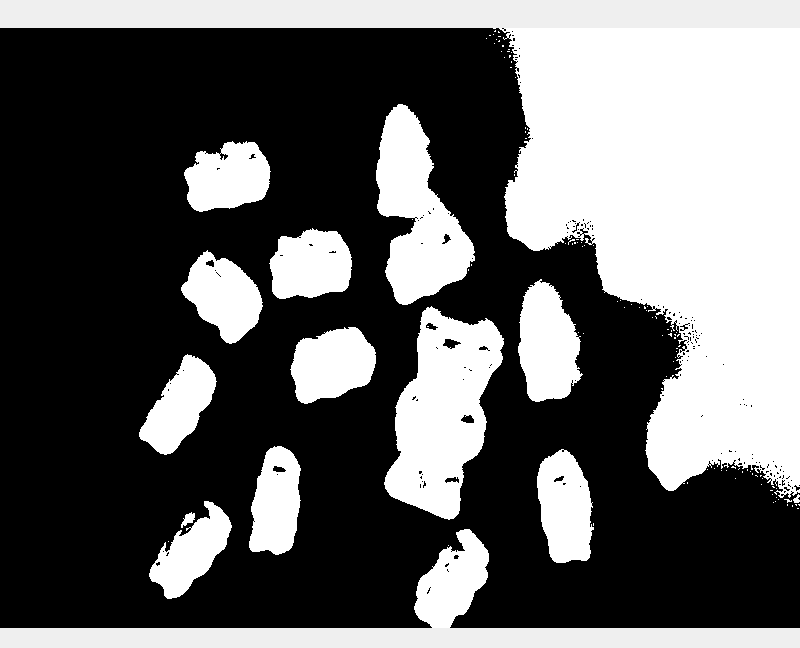
\includegraphics[width=0.6\textwidth, keepaspectratio]{otsu.png}\\
  $T = 145$
\end{figure}

\newpage

\subsection*{Teil 2. Region Growing}
Das Region Growing Vefahren ist in der Funktion \textbf{region\_growing} (main.py Zeile 107) implementiert.
Diese Funktion bekommt das Eingabebild und die Position des Saatpixels übergeben und iteriert über jedes Pixel in dem Bild und überprüft ob dieses Pixel Teil der Region ist. Ist der Pixel Teil der Region iteriert sie über jeden benachbarten Pixel und überprüft ob der Wert dieses Nachbarpixels innerhalb einer spezifischen Varianz zum Saatpixel liegt, ist dies der Fall wird der Pixel zu der Region hinzugefügt. Dies wird so lange wiederholt bis sich das Ausgabebild nicht mehr verändert hat.

\subsubsection*{Ergebnisbilder}
\begin{figure}[H]
  \centering
  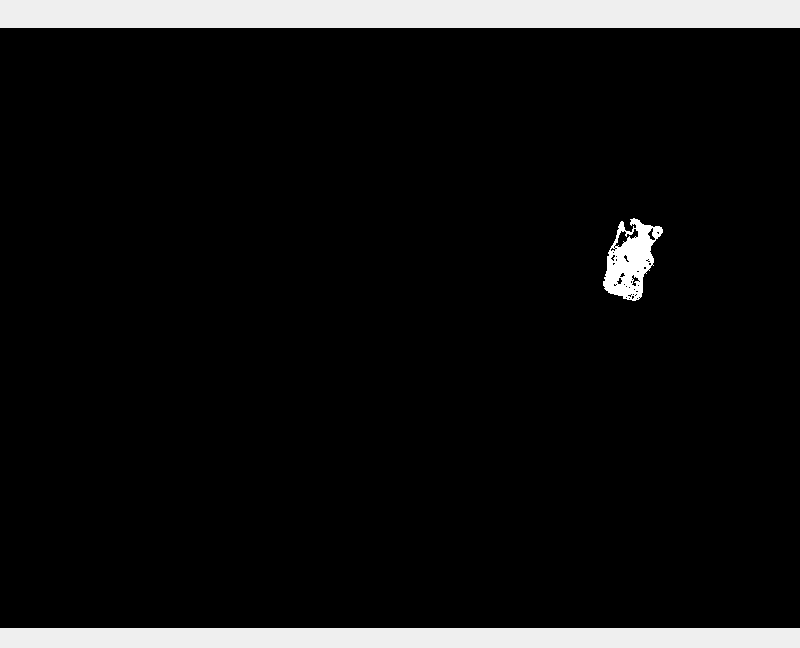
\includegraphics[width=0.6\textwidth, keepaspectratio]{region_growing_1.png}\\
  Saatpixel im zweiten Gummibärchen von rechts
\end{figure}
\begin{figure}[H]
  \centering
  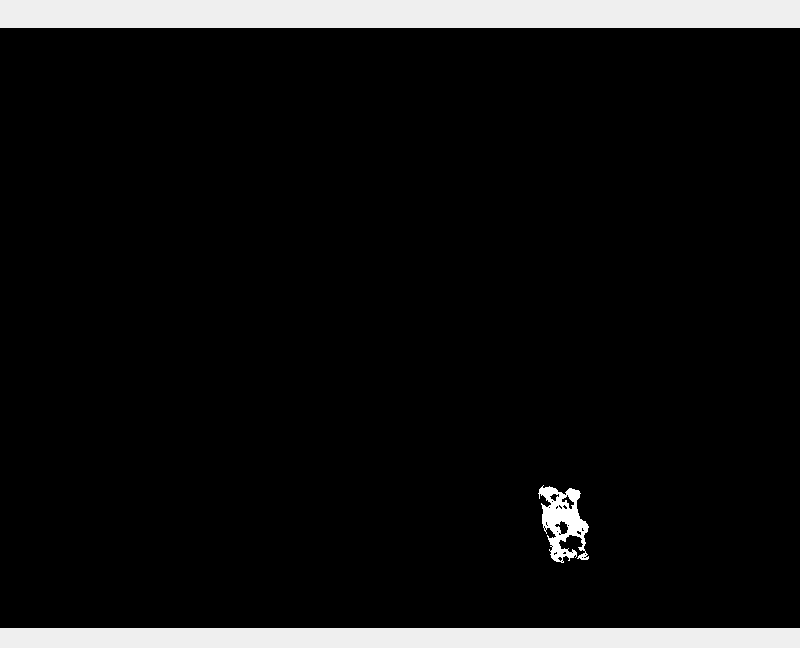
\includegraphics[width=0.6\textwidth, keepaspectratio]{region_growing_2.png}\\
  Saatpixel im dritten Gummibärchen von unten
\end{figure}
\begin{figure}[H]
  \centering
  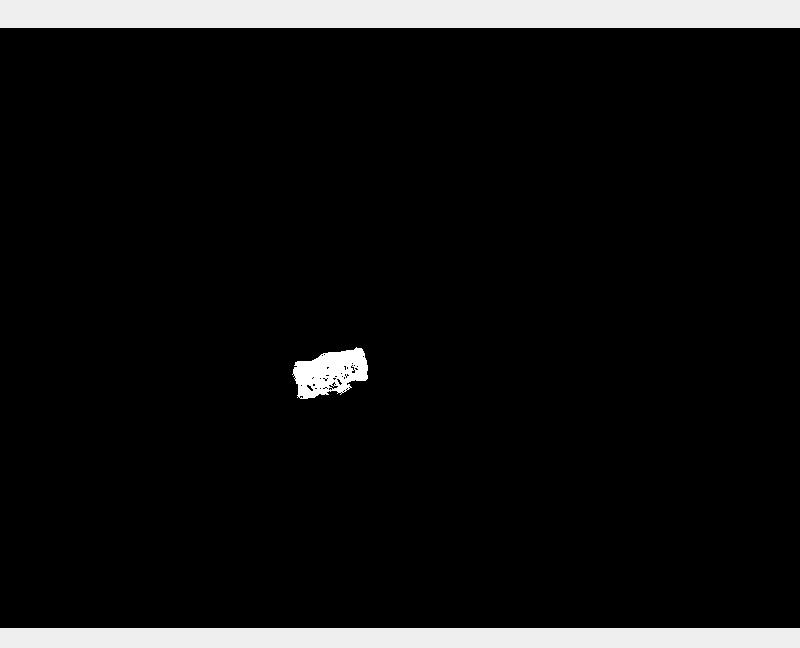
\includegraphics[width=0.6\textwidth, keepaspectratio]{region_growing_3.png}\\
  Saatpixel im dunkelsten Gummibärchen
\end{figure}

\end{document}
